% 例 1：等腰梯形 AD=4, BC=10, ∠B=60°，作两高 AE、DF
\documentclass[tikz,border=4pt]{standalone}
\usepackage{ctex}
\usepackage{amsmath}
\usetikzlibrary{calc, decorations.markings}
\begin{document}
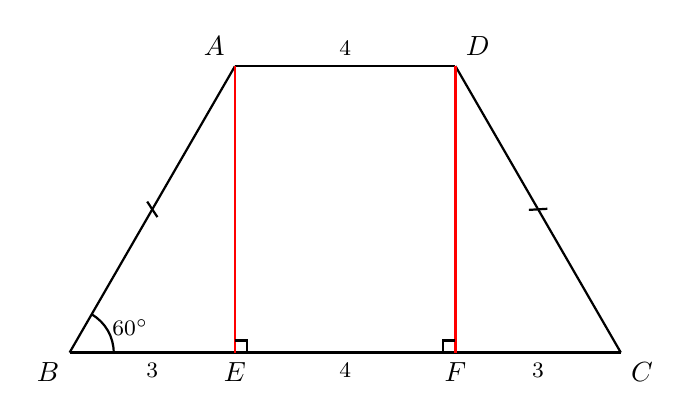
\begin{tikzpicture}[
  scale=0.7, thick,
  tickone/.style={postaction={decorate, decoration={markings,
    mark=at position 0.5 with {\draw (-1.5pt,-3pt) -- (1.5pt,3pt);}}}},
]
  % 等腰梯形：BC=10 (从 0 到 10)；上底 AD=4 居中，AD 在 y=h=3√3≈5.196；BE=FC=3
  \coordinate (B) at (0,0);
  \coordinate (C) at (10,0);
  \coordinate (E) at (3,0);
  \coordinate (F) at (7,0);
  \coordinate (A) at (3,5.196);
  \coordinate (D) at (7,5.196);

  \draw[tickone] (A)--(B);
  \draw[tickone] (D)--(C);
  \draw (A)--(D);
  \draw (B)--(C);

  \draw[red] (A)--(E);
  \draw[red] (D)--(F);
  \draw (E) ++(0.22,0) -- ++(0,0.22) -- ++(-0.22,0);
  \draw (F) ++(-0.22,0) -- ++(0,0.22) -- ++(0.22,0);

  \node[above left]  at (A) {$A$};
  \node[above right] at (D) {$D$};
  \node[below left]  at (B) {$B$};
  \node[below right] at (C) {$C$};
  \node[below] at (E) {$E$};
  \node[below] at (F) {$F$};
  \node[above] at (5,5.196) {\footnotesize $4$};
  \node[below] at (1.5,0)  {\footnotesize $3$};
  \node[below] at (5,0)    {\footnotesize $4$};
  \node[below] at (8.5,0)  {\footnotesize $3$};
  % 60° 角弧
  \draw (0.8,0) arc[start angle=0, end angle=60, radius=0.8];
  \node at (1.1,0.45) {\footnotesize $60^\circ$};
\end{tikzpicture}
\end{document}
